\documentclass[aspectratio=169,11pt]{beamer}

% ─── Clean minimal theme ────────────────────────────────────────────────────
\usetheme{default}
\usecolortheme{dove}
\usefonttheme{professionalfonts}
\setbeamertemplate{navigation symbols}{}
\setbeamertemplate{footline}[frame number]
\setbeamertemplate{frametitle}{%
  \vspace{0.4em}\insertframetitle\par
}

% Colors
\definecolor{accent}{HTML}{2171B5}
\definecolor{darktext}{HTML}{333333}
\definecolor{lightbg}{HTML}{F0F4F8}
\definecolor{greenaccent}{HTML}{2E7D32}
\definecolor{redaccent}{HTML}{C62828}
\definecolor{orangeaccent}{HTML}{E65100}
\setbeamercolor{title}{fg=accent}
\setbeamercolor{frametitle}{fg=accent}
\setbeamercolor{structure}{fg=accent}
\setbeamercolor{normal text}{fg=darktext}
\setbeamercolor{itemize item}{fg=accent}
\setbeamercolor{footline}{fg=gray}
\setbeamerfont{title}{series=\bfseries,size=\Large}
\setbeamerfont{frametitle}{series=\bfseries,size=\large}

% Packages
\usepackage{graphicx}
\usepackage{booktabs}
\usepackage{amsmath,amssymb}
\usepackage{mathtools}
\usepackage{tikz}
\usetikzlibrary{arrows.meta,positioning,calc,decorations.pathreplacing,shapes.geometric}
\usepackage{algorithm}
\usepackage{algorithmic}

\graphicspath{{figures/}}

\newcommand{\E}{\mathbb{E}}
\newcommand{\KL}{\mathrm{KL}}
\newcommand{\Var}{\mathrm{Var}}
\DeclareMathOperator{\Cov}{Cov}

\title{MALA-Guided Mirror Descent\\for Diffusion Policies}
\subtitle{Inference-Time Tilting with Recursive Self-Improvement}
\author{Philip Nielsen}
\date{Spring 2026}

\begin{document}

% ═══════════════════════════════════════════════════════════════════════════════
\begin{frame}
\titlepage
\end{frame}

% ═══════════════════════════════════════════════════════════════════════════════
\begin{frame}{Outline}
\tableofcontents
\end{frame}

% ═══════════════════════════════════════════════════════════════════════════════
\section{Motivation: Inference-Time Compute}

% ═══════════════════════════════════════════════════════════════════════════════
\begin{frame}{Why Inference-Time Compute?}
\textbf{Lesson from LLMs:} Thinking models (o1, DeepSeek-R1) scale compute \emph{at inference time} to solve harder problems.

\pause
\medskip
\textbf{Standard RL amortizes everything into the policy.}
\begin{itemize}\setlength\itemsep{4pt}
  \item The policy network must compress all decision-making into a single forward pass.
  \item No mechanism to ``think harder'' on novel or difficult states.
  \item Some things are better learned on the fly.
\end{itemize}

\pause
\medskip
\textbf{Inference-time methods unlock:}
\begin{itemize}\setlength\itemsep{4pt}
  \item \textcolor{accent}{Scalable compute}: more steps $\Rightarrow$ better actions
  \item \textcolor{accent}{Planning}: multi-step lookahead via composition with world models
  \item \textcolor{accent}{Adaptability}: adjust to new objectives without retraining
\end{itemize}
\end{frame}

% ═══════════════════════════════════════════════════════════════════════════════
\begin{frame}{The MPC--RL Spectrum}
\begin{center}
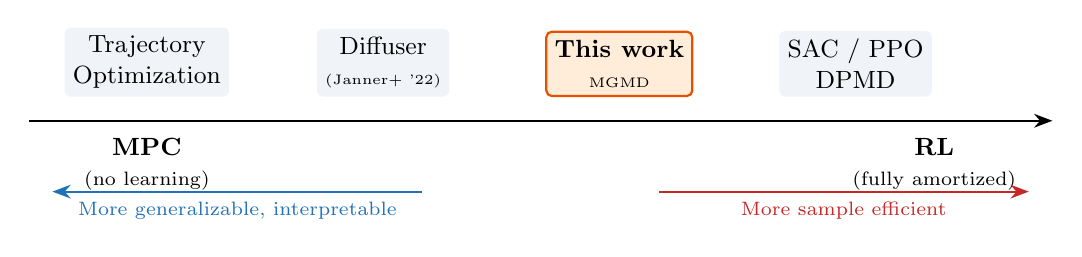
\begin{tikzpicture}[>=Stealth, font=\small]
  % Axis
  \draw[thick, ->] (0,0) -- (13,0);
  % Labels
  \node[below, align=center] at (1.5,-0.1) {\textbf{MPC}\\{\scriptsize (no learning)}};
  \node[below, align=center] at (11.5,-0.1) {\textbf{RL}\\{\scriptsize (fully amortized)}};

  % Ticks and methods
  \node[above, align=center, fill=lightbg, rounded corners=2pt, inner sep=3pt] at (1.5,0.3) {Trajectory\\Optimization};
  \node[above, align=center, fill=lightbg, rounded corners=2pt, inner sep=3pt] at (4.5,0.3) {Diffuser\\{\tiny (Janner+ '22)}};
  \node[above, align=center, fill=orange!15, rounded corners=2pt, inner sep=3pt, draw=orangeaccent, thick] at (7.5,0.3) {\textbf{This work}\\{\tiny MGMD}};
  \node[above, align=center, fill=lightbg, rounded corners=2pt, inner sep=3pt] at (10.5,0.3) {SAC / PPO\\DPMD};

  % Arrows showing properties
  \draw[thick, accent, <-] (0.3,-0.9) -- (5,-0.9) node[midway, below, font=\scriptsize] {More generalizable, interpretable};
  \draw[thick, redaccent, <-] (12.7,-0.9) -- (8,-0.9) node[midway, below, font=\scriptsize] {More sample efficient};
\end{tikzpicture}
\end{center}

\pause
\vspace{0.3cm}
\textbf{Key tension:}
\begin{itemize}
  \item MPC: actions from optimization $\Rightarrow$ generalizable, interpretable, but no policy to improve
  \item RL: actions from a learned policy $\Rightarrow$ fast inference, but no scaling mechanism
  \item \textbf{Goal:} MPC-style inference-time optimization that \emph{also} improves the base policy
\end{itemize}
\end{frame}

% ═══════════════════════════════════════════════════════════════════════════════
\begin{frame}{Prior Work: Inference-Time Scaling for Actions}
\textbf{Diffuser} {\small (Janner, Du, Tenenbaum, Levine --- ICML 2022)}
\begin{itemize}\setlength\itemsep{3pt}
  \item Diffusion model over entire state-action trajectories
  \item Classifier-guided sampling $\Rightarrow$ plans toward high reward
  \item One-shot solutions to mazes via test-time guidance
  \item \textcolor{redaccent}{Limitation:} offline only, no recursive self-improvement
\end{itemize}

\pause
\medskip
\textbf{Inference-time Scaling via Classical Search} {\small (Zhang et al.\ 2025)}
\begin{itemize}\setlength\itemsep{3pt}
  \item Annealed Langevin MCMC for local search in diffusion models
  \item BFS/DFS tree search for global exploration
  \item Applied to planning, offline RL, and image generation
  \item \textcolor{redaccent}{Limitation:} no recursive self-improvement demonstrated
\end{itemize}

\pause
\medskip
\textbf{Neither has demonstrated recursive self-improvement:} \\
improved actions are not distilled back into the base policy.
\end{frame}

% ═══════════════════════════════════════════════════════════════════════════════
\begin{frame}{Our Goal}
\begin{center}
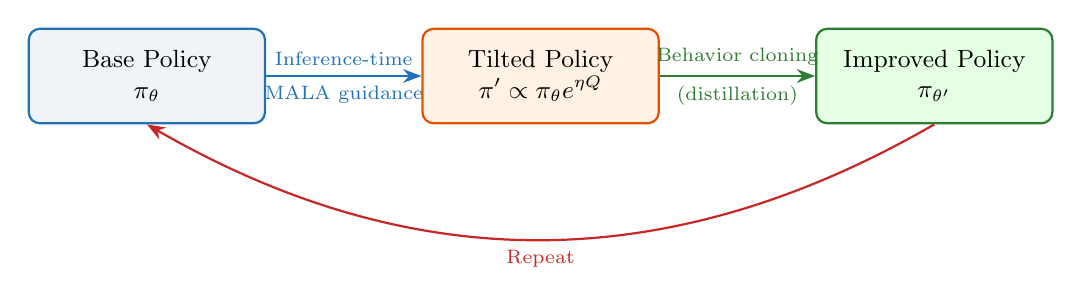
\begin{tikzpicture}[>=Stealth, font=\small,
    box/.style={draw=accent, thick, rounded corners=4pt, fill=lightbg,
                minimum width=3cm, minimum height=1.2cm, align=center}]

  \node[box] (base) at (0,0) {Base Policy\\$\pi_\theta$};
  \node[box, fill=orange!10, draw=orangeaccent] (tilt) at (5,0) {Tilted Policy\\$\pi' \propto \pi_\theta e^{\eta Q}$};
  \node[box, fill=green!10, draw=greenaccent] (improved) at (10,0) {Improved Policy\\$\pi_{\theta'}$};

  \draw[->, thick, accent] (base) -- (tilt)
    node[midway, above, font=\scriptsize] {Inference-time}
    node[midway, below, font=\scriptsize] {MALA guidance};
  \draw[->, thick, greenaccent] (tilt) -- (improved)
    node[midway, above, font=\scriptsize] {Behavior cloning}
    node[midway, below, font=\scriptsize] {(distillation)};
  \draw[->, thick, redaccent, bend left=30] (improved.south) to
    node[midway, below, font=\scriptsize] {Repeat} (base.south);
\end{tikzpicture}
\end{center}

\pause
\vspace{0.3cm}
\textbf{Requirements:}
\begin{enumerate}\setlength\itemsep{4pt}
  \item Actions must come from a \textbf{well-defined tilted distribution} $\pi' \propto \pi_\theta \cdot e^{\eta Q}$ (not just high-Q filtered samples)
  \item The tilted distribution must be a \textbf{sensible policy update} (mirror descent)
  \item \textbf{Diffusion policies}: admit gradient-based guidance at inference time
\end{enumerate}
\end{frame}

% ═══════════════════════════════════════════════════════════════════════════════
\section{Why Diffusion Policies?}

% ═══════════════════════════════════════════════════════════════════════════════
\begin{frame}{Why Not Gaussian Policies?}
\textbf{Standard approach:} $\pi_\theta(a|s) = \mathcal{N}(\mu_\theta(s), \sigma_\theta(s))$

\begin{itemize}\setlength\itemsep{6pt}
  \item \textcolor{greenaccent}{Pro:} Simple, fast sampling; policy gradient is cheap ($\nabla_\theta \log \pi_\theta$ in closed form)
  \item \textcolor{redaccent}{Con:} Unimodal --- cannot represent multimodal action distributions
  \item \textcolor{redaccent}{Con:} No mechanism for inference-time guidance
\end{itemize}

\pause
\medskip
\textbf{Diffusion policies:} $\pi_\theta(a|s)$ via iterative denoising
\begin{itemize}\setlength\itemsep{6pt}
  \item \textcolor{greenaccent}{Pro:} Expressive --- can represent arbitrary distributions
  \item \textcolor{greenaccent}{Pro:} Admit guidance at inference time (the whole point!)
  \item \textcolor{redaccent}{Con:} Policy gradient would require backprop through the full denoising chain\\
        $\Rightarrow$ many forward/backward passes per update $\Rightarrow$ expensive \& inaccurate
  \item \textcolor{accent}{Solution:} Mirror descent with behavior cloning + inference-time tilting
\end{itemize}
\end{frame}

% ═══════════════════════════════════════════════════════════════════════════════
\section{Guidance Methods: From Na\"ive to MALA}

% ═══════════════════════════════════════════════════════════════════════════════
\begin{frame}{Energy Guidance for Diffusion Policies}
\textbf{Goal:} Sample actions from the \emph{tilted} distribution
\[
  \pi'(a|s) \;\propto\; \pi_\theta(a|s) \cdot e^{\eta\, Q(s,a)}
\]

\pause
\medskip
\textbf{Energy view:} If $\pi_\theta(a|s) \propto e^{-E_\theta(a,s)}$, then:
\[
  \pi'(a|s) \;\propto\; e^{-\big(E_\theta(a,s)\;-\;\eta\, Q(s,a)\big)}
  \;=\; e^{-E^{\mathrm{total}}(a,s)}
\]

\pause
\medskip
\textbf{Guided score:}
\[
  \nabla_a \log \pi'(a|s) = \underbrace{\nabla_a \log \pi_\theta(a|s)}_{\text{base score}} + \underbrace{\eta\, \nabla_a Q(s,a)}_{\text{guidance}}
\]

\pause
\begin{itemize}\setlength\itemsep{4pt}
  \item This is exact \textbf{at $t=0$} (clean data level)
  \item At intermediate diffusion levels $t > 0$, simply adding $\eta \nabla Q$ to the noisy score is \textbf{not correct} --- we will return to this
  \item First: how do we get $\nabla_a Q$ during the reverse process?
\end{itemize}
\end{frame}

% ═══════════════════════════════════════════════════════════════════════════════
\begin{frame}{Training-Free Guidance (TFG) via Tweedie Estimates}
\textbf{Idea:} Use the Tweedie estimate $\hat{a}_0$ and a \emph{clean} critic $Q(s, \hat{a}_0)$.

\pause
\medskip
At noise level $t$, given noisy $a_t$ and noise prediction $\epsilon_\theta(a_t, s, t)$:
\[
  \hat{a}_0 = \frac{a_t - \sqrt{1 - \bar\alpha_t}\;\epsilon_\theta(a_t,s,t)}{\sqrt{\bar\alpha_t}}
\]

\pause
Modify the noise prediction:
\[
  \epsilon_{\text{guided}} = \epsilon_\theta - \eta \sigma_t \nabla_{a_t} Q(s, \hat{a}_0(a_t))
\]

\pause
\begin{itemize}\setlength\itemsep{4pt}
  \item \textcolor{greenaccent}{Stronger signal} than noise-conditional classifier guidance
  \item Used in Diffuser (Janner et al.\ 2022) for trajectory planning
  \item \textcolor{redaccent}{Problem:} the guided samples don't target a specific distribution
  \item The resulting ``policy'' may be overly collapsed
  \item \textcolor{redaccent}{No recursive self-improvement} demonstrated via distillation
\end{itemize}
\end{frame}

% ═══════════════════════════════════════════════════════════════════════════════
\begin{frame}{The Reduce, Reuse, Recycle Insight}
{\small Du, Durkan, Strudel, Tenenbaum, Dieleman, Fergus, Sohl-Dickstein, Doucet, Grathwohl (ICML 2023)}

\pause
\medskip
\textbf{At $t=0$ (clean),} na\"ive score summation \emph{is} the score of the tilted distribution:
\[
  \nabla_a \log \tilde{p}_0(a|s) = \nabla_a \log p_0(a|s) + \eta \nabla_a Q(s,a) = \nabla_a \log\!\big[p_0(a|s)\,e^{\eta Q(s,a)}\big]
\]

\pause
\textbf{At $t > 0$ (noisy),} the correct tilted marginal involves an intractable integral:
\[
  \tilde{p}_t(a_t|s) = \int p_{t|0}(a_t | a_0)\, \tilde{p}_0(a_0|s)\, da_0
  \quad\Rightarrow\quad
  \nabla_{a_t}\!\log \tilde{p}_t \;\neq\; \nabla_{a_t}\!\log p_t + \eta\nabla_{a_t} Q(s,\hat{a}_0)
\]
Na\"ive score summation does \emph{not} correspond to the reverse of any valid noising process.

\pause
\medskip
\textbf{Solution:} Treat the combined score as defining an \textbf{energy-based model} at each noise level, and use \textbf{MCMC} to sample from it.

\pause
\smallskip
\begin{center}
\fcolorbox{accent}{lightbg}{\parbox{0.85\textwidth}{\centering
The sequence of EBMs smoothly interpolates between a Gaussian ($t{=}T$) and the exact tilted distribution ($t{=}0$). With enough MCMC steps at each level, we converge to the correct marginal.
}}
\end{center}
\end{frame}

% ═══════════════════════════════════════════════════════════════════════════════
\begin{frame}{From Langevin Dynamics to MALA}
\textbf{Langevin dynamics} at noise level $t$ with total energy $E_t(a_t)$:
\[
  a_t' = a_t - \eta_t \nabla_{a_t} E_t(a_t) + \sqrt{2\eta_t}\; z, \quad z \sim \mathcal{N}(0,I)
\]

\pause
In the limit of $\eta_t \to 0$ and $\infty$ steps, samples converge to:
\[
  p(a_t) \;\propto\; \exp\!\big({-E_t(a_t)}\big)
\]
In practice, finite $\eta_t$ introduces bias.

\pause
\medskip
\textbf{MALA} (Metropolis-Adjusted Langevin Algorithm) adds accept/reject:
\begin{enumerate}\setlength\itemsep{3pt}
  \item \textbf{Propose:} $a_t' = a_t - \eta_t \nabla E_t(a_t) + \sqrt{2\eta_t}\, z$
  \item \textbf{Accept/reject:} with MH ratio $\alpha = \min\!\big(1,\; \frac{p(a_t')}{p(a_t)} \cdot \frac{q(a_t|a_t')}{q(a_t'|a_t)}\big)$
\end{enumerate}

\pause
\medskip
\textcolor{redaccent}{\textbf{Problem:}} MH requires the \emph{density ratio} $p(a_t')/p(a_t)$. \\
Scores alone ($\nabla \log p$) don't give us this.

\pause
\medskip
\textcolor{greenaccent}{\textbf{Solution:}} \textbf{Energy-based parameterization} of the diffusion model!
\end{frame}

% ═══════════════════════════════════════════════════════════════════════════════
\begin{frame}{Energy-Based Parameterization}
\textbf{Standard diffusion:} network predicts noise $\epsilon_\theta(a_t, s, t)$ \\
$\Rightarrow$ gives us the \emph{score} $\nabla_{a_t} \log p_t(a_t|s)$, but not the density

\pause
\medskip
\textbf{Energy parameterization:} network outputs a scalar $E_\theta(a_t, s, t)$
\[
  \text{Score} = \nabla_{a_t} E_\theta(a_t, s, t)
\]
Trained the same way (denoising score matching), but via the input-output gradient.

\pause
\medskip
\textbf{Total energy at noise level $t$:}
\[
  E_t^{\text{total}}(a_t, s) = \underbrace{E_\theta(a_t, s, t)}_{\text{base policy energy}} - \underbrace{\eta_t \cdot Q\big(s, \hat{a}_0(a_t)\big)}_{\text{critic via Tweedie estimate}}
\]

\pause
\medskip
Now the MH acceptance ratio is computable:
\[
  \frac{p(a_t')}{p(a_t)} = \exp\!\Big(E_t^{\text{total}}(a_t, s) - E_t^{\text{total}}(a_t', s)\Big)
\]

\pause
\textcolor{accent}{$\Rightarrow$ We can do proper MALA at each diffusion level!}
\end{frame}

% ═══════════════════════════════════════════════════════════════════════════════
\section{The MGMD Algorithm}

% ═══════════════════════════════════════════════════════════════════════════════
\begin{frame}{MGMD: Putting It All Together}
\begin{center}
\resizebox{0.95\textwidth}{!}{%
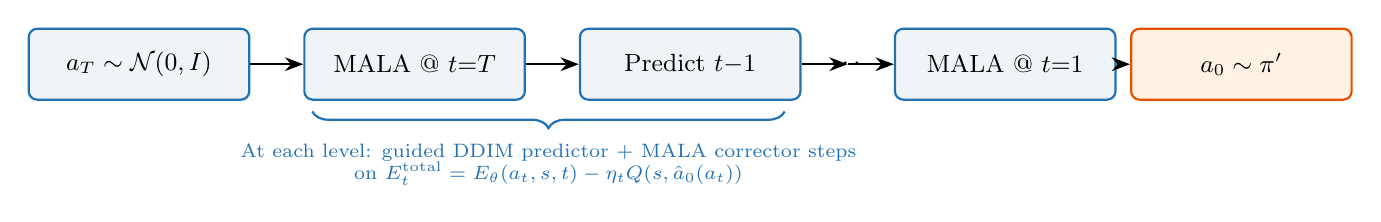
\begin{tikzpicture}[>=Stealth, font=\small,
    stp/.style={draw=accent, thick, rounded corners=3pt, fill=lightbg,
                 minimum width=2.8cm, minimum height=0.9cm, align=center}]

  % Reverse diffusion chain
  \node[stp] (tT) at (0,0) {$a_T \sim \mathcal{N}(0,I)$};
  \node[stp] (mT) at (3.5,0) {MALA @ $t{=}T$};
  \node[stp] (pT) at (7,0) {Predict $t{-}1$};
  \node at (9,0) {$\cdots$};
  \node[stp] (m1) at (11,0) {MALA @ $t{=}1$};
  \node[stp, fill=orange!10, draw=orangeaccent] (a0) at (14,0) {$a_0 \sim \pi'$};

  \draw[->, thick] (tT) -- (mT);
  \draw[->, thick] (mT) -- (pT);
  \draw[->, thick] (pT) -- (9,0);
  \draw[->, thick] (9,0) -- (m1);
  \draw[->, thick] (m1) -- (a0);

  % MALA detail
  \draw[decorate, decoration={brace, amplitude=6pt, mirror}, thick, accent]
    (2.2,-0.6) -- (8.2,-0.6)
    node[midway, below=8pt, align=center, font=\scriptsize] {
      At each level: guided DDIM predictor + MALA corrector steps\\
      on $E_t^{\text{total}} = E_\theta(a_t,s,t) - \eta_t Q(s, \hat{a}_0(a_t))$
    };
\end{tikzpicture}%
}
\end{center}

\pause
\vspace{0.2cm}
\textbf{Training loop} (constant-weight behavior cloning):
\begin{enumerate}\setlength\itemsep{3pt}
  \item Sample action $a \sim \pi'(\cdot|s)$ using MALA-guided diffusion
  \item Execute $a$ in environment, observe $(s, a, r, s')$
  \item Store in replay buffer; train $Q$ by TD learning
  \item Train $\pi_\theta$ by \textbf{uniform-weight} denoising score matching on replay
  \item[$\Rightarrow$] No $Q$-reweighting in training loss --- all critic signal at inference time
\end{enumerate}
\end{frame}

% ═══════════════════════════════════════════════════════════════════════════════
\begin{frame}{Algorithm: MALA-Guided Sampling}
\textbf{For each diffusion level $t = T, \ldots, 1$:}
\smallskip

\textbf{1. Guided predictor step:}
\begin{itemize}\setlength\itemsep{2pt}
  \item[\tiny$\blacktriangleright$] Compute $\epsilon_\theta(a_t, s, t)$
  \item[\tiny$\blacktriangleright$] Tweedie: $\hat{a}_0 = \frac{a_t - \sqrt{1-\bar\alpha_t}\,\epsilon_\theta}{\sqrt{\bar\alpha_t}}$, \quad clip $\hat{a}_0$ to $[\text{-}r, r]$
  \item[\tiny$\blacktriangleright$] Guided noise: $\epsilon' = \epsilon_\theta - \eta_t \sigma_t \nabla_{a_t} Q(s, \hat{a}_0)$
  \item[\tiny$\blacktriangleright$] DDIM step: $a_{t-1} = \mu(a_t, \epsilon')$ \quad {\small (deterministic, no added noise)}
\end{itemize}

\smallskip
\textbf{2. MALA corrector} ($K$ steps at level $t{-}1$):
\begin{itemize}\setlength\itemsep{2pt}
  \item[\tiny$\blacktriangleright$] Compute total energy $E_{t-1}^{\text{total}}(a, s) = E_\theta(a,s,t{-}1) - \eta_{t-1} Q(s, \hat{a}_0(a))$
  \item[\tiny$\blacktriangleright$] Propose: $a' = a - \eta\nabla E_{t-1}^{\text{total}} + \sqrt{2\eta}\,z$
  \item[\tiny$\blacktriangleright$] MH accept/reject using energy ratio
  \item[\tiny$\blacktriangleright$] Adapt $\eta$ toward 57.4\% acceptance rate (per noise level)
\end{itemize}
\end{frame}

% ═══════════════════════════════════════════════════════════════════════════════
\section{Theoretical Foundations: Self-Consistent Policy Updates}

% ═══════════════════════════════════════════════════════════════════════════════
\begin{frame}{Why the Exponential Tilt?}
The mirror descent update is:
\[
  \pi_{k+1}(a \mid s) \;\propto\; \pi_k(a \mid s)\,\exp\!\big(\eta\, A_k(s,a)\big)
\]
\textbf{Standard derivation:} KL-regularized optimization $\Rightarrow$ exponential form as a consequence of the Bregman divergence.

\pause
\medskip
\textbf{Alternative question:} Is there a \emph{structural} reason why this update is the right one?

\pause
\medskip
\textbf{Answer: Yes.} The exponential tilt is the \emph{unique} update satisfying a natural self-consistency property.
\end{frame}

% ═══════════════════════════════════════════════════════════════════════════════
\begin{frame}{Self-Consistency of Mirror Descent}
\smallskip
\textbf{Axiom}\; \textcolor{accent}{(C)}\; \textbf{Compositionality:}\;
$w\!\bigl(\textstyle\prod_t p_t,\;\sum_t A_t\bigr) = \prod_t w(p_t, A_t)$

\pause
\smallskip
Set all but one factor to $(1,0)$, noting $w(1,0)=1$:
\[
  w(p,A) = w(p,0)\;\cdot\; w(1,A)
\]
\pause
Substitute back into \textcolor{accent}{(C)} and cancel $\prod p_t$:
\begin{align*}
  w(p,0)&:\quad f(p_1 p_2) = f(p_1)\,f(p_2) &&\Longrightarrow\quad f(p) = p^\alpha \\
  w(1,A)&:\quad h(A_1+A_2) = h(A_1)\,h(A_2) &&\Longrightarrow\quad h(A) = e^{\eta A}
\end{align*}
\vspace{-0.4cm}

From compositionality alone: $\;w(p,A) = p^\alpha\, e^{\eta A}$.

\pause
\medskip
\textbf{Axiom}\; \textcolor{accent}{(N)}\; \textbf{Shift Invariance:}\;
$w(p,\, c) / \sum w(p_{a'},c) = p$\;\; (flat advantage $\Rightarrow$ no change)\;\; $\Longrightarrow\;\alpha = 1$.

\pause
\smallskip
\begin{center}
\fcolorbox{accent}{white}{\;\;$\displaystyle
  w(p,A) = p\,e^{\eta A}
  \qquad\Longrightarrow\qquad
  \pi'(a\!\mid\!s)\;\propto\;\pi(a\!\mid\!s)\,e^{\eta\, A(s,a)}
$\;\;}
\end{center}
\vspace{-0.15cm}
\small\textcolor{gray}{Tilting a trajectory by its total advantage = tilting each step independently. The exponential tilt is the unique update with this property.}
\end{frame}

% ═══════════════════════════════════════════════════════════════════════════════
\begin{frame}{Structural Consequences}

\textbf{1. $\eta$ must be a global scalar} (not state-dependent).
\begin{itemize}
  \item A state-dependent $\eta(s)$ would break trajectory-level compositionality.
  \item The step size can vary across iterations, but must be shared across states.
\end{itemize}

\pause
\medskip
\textbf{2. Any additional signal must aggregate additively.}
\begin{itemize}
  \item Advantage: $\sum_t A_t$ $\checkmark$
  \item Advantage variance: $\sum_t \sigma^2_t$ $\checkmark$ (under conditional independence)
  \item The self-consistent joint update: $w(p, A, \sigma^2) = p \cdot \exp(c_1 A + c_2 \sigma^2)$
\end{itemize}

\pause
\medskip
\textbf{3. Without shift invariance:} the general family is $w(p,A) = p^\alpha e^{\eta A}$, corresponding to $\alpha$-divergence (R\'enyi) mirror descent.
\end{frame}

% ═══════════════════════════════════════════════════════════════════════════════
\begin{frame}{Adaptive $\eta$ via KL Budget}
\smallskip
Self-consistency $\Rightarrow$ $\eta_k$ must be a \textbf{single global scalar} per update (not state-dependent).

\pause
\medskip
\textbf{KL expansion.}\; For the tilted policy $\pi_\eta(a)\propto \pi(a)\,e^{\eta A(a)}$:
\vspace{-0.15cm}
\[
  \KL(\pi_\eta\,\|\,\pi)
  \;=\; \eta\,\E_{\pi_\eta}[A] - \log\E_\pi[e^{\eta A}]
  \;=\; \tfrac{\eta^2}{2}\,\Var_\pi(A) + O(\eta^3).
\]
\vspace{-0.3cm}

\pause
Target a fixed KL budget $\Delta$, solve $\E_{s \sim d_{\pi_k}}[\KL(\pi_{\eta_k}\|\pi_k)]=\Delta$:
\vspace{-0.1cm}
\[
  \boxed{\;\eta_k = \sqrt{\frac{2\,\Delta}{\E_{s \sim d_{\pi_k}}[\Var_{\pi_k}(A_k)]}}\;}
\]
\vspace{-0.3cm}

\pause
\textbf{Scale invariance.}\; $A\mapsto cA$ $\;\Rightarrow\;$ $\Var\mapsto c^2\Var$ $\;\Rightarrow\;$ $\eta\mapsto\eta/c$ $\;\Rightarrow\;$ $\eta A$ unchanged.

\pause
\medskip
Substituting back: $\;\pi_{k+1}(a|s) \propto \pi_k(a|s)\exp\!\Big(A_k(s,a)\sqrt{2\Delta\, /\, \E_s[\Var(A_k)]}\Big)$

\smallskip
\small\textcolor{gray}{The KL budget does not add a free parameter --- its sole consequence is variance normalization of the advantage.}
\end{frame}

% ═══════════════════════════════════════════════════════════════════════════════
\begin{frame}{Optimal $\eta^*$ via Distribution Shift}
\small
The KL budget treats each state independently. In the MDP, the policy changes at every state, so $Q$-values become stale. Expand the true improvement to second order:

\pause
\vspace{-0.1cm}
\[
  \Delta V(s;\eta) = V^{\pi_\eta}(s) - V^\pi(s)
\]
Using $Q^{\pi_\eta} = Q^\pi + \gamma\,\E_{s'|s,a}[\Delta V(s';\eta)]$ and expanding in $\eta$:
\vspace{-0.1cm}
\[
  \E_{s\sim d_\pi}[\Delta V(s;\eta)] \;\approx\; \eta\, \bar{u}_1 + \eta^2\, \bar{u}_2
\]

\pause
\vspace{-0.1cm}
where (averaging over $s \sim d_\pi$, $a \sim \pi$):
\vspace{-0.1cm}
\begin{align*}
  \bar{u}_1 &= \E_s\!\left[\Var_a(A^\pi)\right] & &\text{\small (advantage variance --- first-order gain)}\\
  \bar{u}_2 &= \E_s\!\left[\tfrac{1}{2}\E_a[(A^\pi)^3] + \gamma\,\Cov_a\!\big(\E_{s'|s,a}[\delta_1(s')],\, A^\pi\big)\right] & &\text{\small (skewness + dist.\ shift)}
\end{align*}

\pause
\vspace{-0.1cm}
$\delta_1(s)$ satisfies a Bellman equation: $\delta_1 = u_1 + \gamma P^\pi \delta_1$, so $\delta_1 = (I - \gamma P^\pi)^{-1} u_1$.

\pause
\medskip
Optimizing the quadratic surrogate:
\[
  \boxed{\;\eta^*_{\text{quad}} = -\frac{\bar{u}_1}{2\,\bar{u}_2}
  = -\frac{
    \E_s[\Var_a(A^\pi)]
  }{
    \E_s[\E_a[(A^\pi)^3]]
    + 2\gamma\,\E_s[\Cov_a(\E_{s'|s,a}[\delta_1(s')],\, A^\pi)]
  }\;}
\]
\vspace{-0.2cm}

\small\textcolor{gray}{The numerator drives improvement; the denominator penalizes via skewness and distribution shift (actions that look good under the old critic may lead to states where the critic is stale).}
\end{frame}

% ═══════════════════════════════════════════════════════════════════════════════
\section{Toward Model-Based Planning}

% ═══════════════════════════════════════════════════════════════════════════════
\begin{frame}{Compositional Guidance via World Models}
\textbf{Current:} Guidance uses a monolithic $Q$-function. \quad
\textbf{Future:} Replace $Q$ with compositional objective:
\vspace{-0.1cm}
\[
  \hat{Q}(s,a) = \E_{s' \sim p_\phi(\cdot|s,a)}\!\left[r_\psi(s,a,s') + \gamma V_\xi(s')\right]
\]
\vspace{-0.4cm}

\pause
\begin{itemize}\setlength\itemsep{2pt}
  \item Dynamics $p_\phi$, reward $r_\psi$, value $V_\xi$ trained separately
  \item Each component has a \emph{stationary} target (except $V$)
  \item As planning horizon grows, reliance on non-stationary $V$ decreases
\end{itemize}

\pause
\smallskip
\textbf{Short-horizon planning} ($H > 1$): \; $\hat{Q}_H = \sum_{h=0}^{H-1} \gamma^h r(s_h, a_h, s_{h+1}) + \gamma^H V(s_H)$

Execute only $a_0$, re-plan from true $s_1$ (MPC-style).

\pause
\smallskip
\textcolor{gray}{\small Preliminary HalfCheetah results: model-based variants train stably but don't yet outperform $Q$-based guidance. Humanoid is next.}
\end{frame}

% ═══════════════════════════════════════════════════════════════════════════════
\begin{frame}{}
\begin{center}
\vspace{2cm}
{\Large\textcolor{accent}{\textbf{Thank you!}}}

\vspace{1cm}
\textbf{Philip Nielsen}\\
\texttt{pnielsen@seas.harvard.edu}

\vspace{0.5cm}
\small Code: \texttt{github.com/pnielsen2/inference\_mirror\_descent}
\end{center}
\end{frame}

\end{document}
